\documentclass[11pt,a4paper,twoside]{article}
\usepackage[english]{babel}
\usepackage[framed,numbered,autolinebreaks,useliterate]{mcode}

\usepackage{amsmath,amssymb,amsfonts,textcomp}

\usepackage{graphicx}
\usepackage{float,flafter}
\usepackage{hyperref}
\usepackage{inputenc}
\usepackage{pdfpages}

\setlength\paperwidth{20.999cm}\setlength\paperheight{29.699cm}\setlength\voffset{-1in}\setlength\hoffset{-1in}\setlength\topmargin{1.499cm}\setlength\headheight{12pt}\setlength\headsep{0cm}\setlength\footskip{1.131cm}\setlength\textheight{25cm}\setlength\oddsidemargin{2.499cm}\setlength\textwidth{16.5cm}

\begin{document}

\begin{center}
\hrule

\vspace{.4cm}
{\bf {\Huge Digital Signal Processing Lab Report}}
\vspace{.2cm}
\end{center}
{\bf Name:\ Yang Chang }  \\
{\bf ID Number:\ 2289206Y} \hspace{\fill} 22 May 2019 \\
\hrule

\section{M1}

\lstinputlisting{m1_1.m}

\begin{figure}[H]
\centering
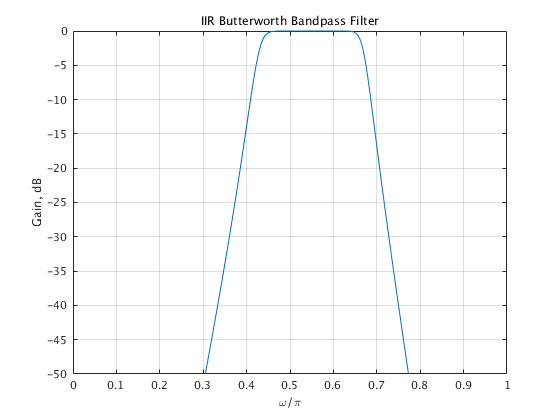
\includegraphics[width=0.8\linewidth]{img/m1}
\caption{Figure of M1}
\label{Figure of M1}
\end{figure}


\section{M2}

\lstinputlisting{m2_1.m}

\lstinputlisting{plot_filter.m}

\begin{figure}[H]
\centering
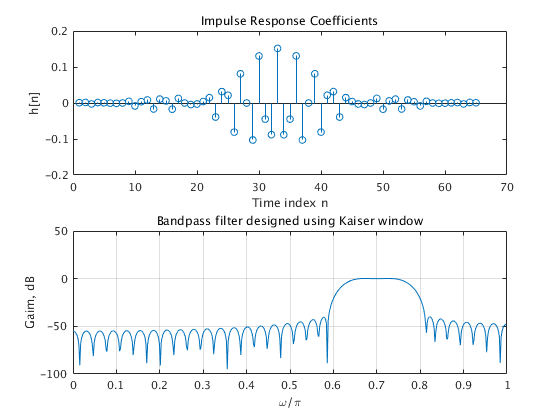
\includegraphics[width=0.8\linewidth]{img/m2_1}
\caption{Figure 1 of M2 (Kaiser)}
\label{Figure 1 of M2}
\end{figure}

\begin{figure}[H]
\centering
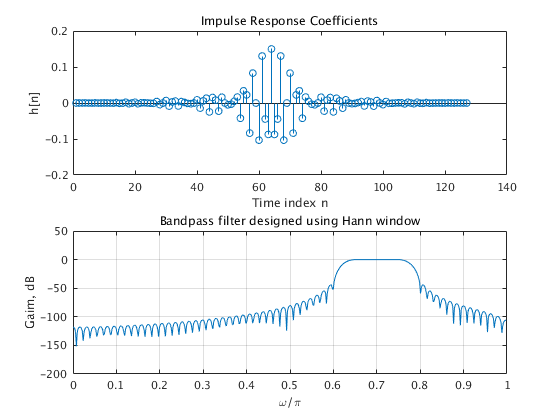
\includegraphics[width=0.8\linewidth]{img/m2_2}
\caption{Figure 2 of M2 (Hann)}
\label{Figure 2 of M2}
\end{figure}

\begin{figure}[H]
\centering
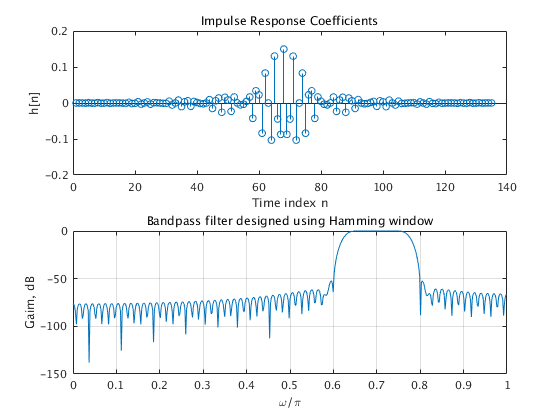
\includegraphics[width=0.8\linewidth]{img/m2_3}
\caption{Figure 3 of M2 (Hamming)}
\label{Figure 3 of M2}
\end{figure}

\end{document}
